\documentclass[tikz]{standalone}

% \usepackage{newtxtext,newtxmath}

% mytikzset
\usepackage{tikz}
\usetikzlibrary{positioning,arrows,shapes,patterns}
\usetikzlibrary{decorations.pathmorphing}
\usetikzlibrary{decorations.pathreplacing}
\usetikzlibrary{decorations.markings}
\usetikzlibrary{shapes.arrows, fadings}
\usetikzlibrary{calc}
\usetikzlibrary{}


\tikzset{
  vector/.style={thick,double,draw=black, postaction={decorate},
    decoration={markings,mark=at position .6 with {\arrow[black,scale=0.4]{triangle 45}}}},
  axial/.style={thick,double,densely dashed,draw=black, postaction={decorate},
    decoration={markings,mark=at position .6 with {\arrow[black,scale=0.4]{triangle 45}}}},
  gluon/.style={decorate, draw=black,
    decoration={coil,aspect=0.3,segment length=5pt,amplitude=3pt}},
  pseudo/.style={thick, dashed, draw=black, postaction={decorate},
    decoration={markings,mark=at position .6 with {\arrow[red,scale=0.5]{triangle 45}}}},
  scalar/.style={thick,draw=black, postaction={decorate},
    decoration={markings,mark=at position .6 with {\arrow[black,scale=0.5]{triangle 45}}}}%,
  % pomeron/.style={thick,draw=black, postaction={decorate},
  % decoration={zigzag,segment length=4,amplitude=.9}}
}

\definecolor{myGreen}{RGB}{0,127,0}

\begin{document}
\nopagecolor
  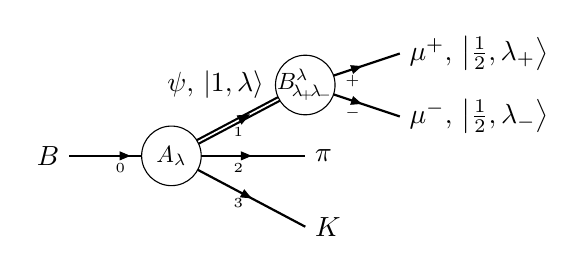
\begin{tikzpicture}[node distance=0.9cm and 1.3cm, baseline=1cm]
    \coordinate[] (c0);
    \coordinate[left=of c0,label= left:{$B$}] (Lamc);
    \coordinate[above right=of c0, xshift=4mm, label={left,xshift=-4mm}:{$\psi,\,\left|1,\lambda\right\rangle$}] (p);
    \coordinate[      right=of c0, xshift=4mm, label=right:{$\pi$}] (pi);
    \coordinate[below right=of c0, xshift=4mm, label=right:{$K$}] (K);

    \coordinate[above right=of p, xshift=-1mm, yshift=-5mm, label=right:{$\mu^+,\,\left|\frac{1}{2},\lambda_+\right\rangle$}] (mu1);
    \coordinate[below right=of p, xshift=-1mm, yshift=+5mm, label=right:{$\mu^-,\,\left|\frac{1}{2},\lambda_-\right\rangle$}] (mu2);


    \draw[scalar]  (Lamc) -- node[yshift=-1.5mm] {\tiny $0$}  (c0);
    \draw[vector]  (c0) -- node[yshift=-1.5mm] {\tiny $1$} (p);
    \draw[scalar]  (c0) -- node[yshift=-1.5mm] {\tiny $2$} (pi);
    \draw[scalar]  (c0) -- node[yshift=-1.5mm] {\tiny $3$} (K);

    \draw[scalar]  (p) -- node[yshift=-1.5mm] {\tiny $+$} (mu1);
    \draw[scalar]  (p) -- node[yshift=-1.5mm] {\tiny $-$} (mu2);

    \draw[black, fill=white] (c0) circle (2.5ex) node[scale=0.85] {$A_{\lambda}$};
    \draw[black, fill=white] (p) circle (2.5ex) node[scale=0.85] {$B^{\lambda}_{\!\lambda_{\!+}\!\lambda_{\!-}}$};
  \end{tikzpicture}
\end{document}
